\documentclass[12pt]{report}
\usepackage[francais]{babel}
\usepackage{lmodern}
\usepackage[a4paper]{geometry}
\usepackage[T1]{fontenc}
\usepackage[utf8]{inputenc}  
\usepackage{moreverb}
\usepackage{amsmath}
\usepackage{amsfonts}
\usepackage{amssymb}
\usepackage{textcomp}
\usepackage{pifont}
\usepackage{geometry}
\usepackage[pdftex]{graphicx}
\usepackage{graphics}
\usepackage{url}
\usepackage{graphicx}
\usepackage{float}
\usepackage{color}
\usepackage[nottoc, notlof, notlot]{tocbibind}
\usepackage[french]{varioref}
\usepackage[Glenn]{fncychap}
\usepackage{pdfpages}

\usepackage[colorlinks=true]{hyperref}
\hypersetup{urlcolor=blue,linkcolor=black,citecolor=black,colorlinks=true}

\usepackage{multicol}

% entête et pied de page
%% \usepackage{fancyhdr} 
%% \pagestyle{fancy}
%% \renewcommand{\chaptermark}[1]{\markboth{#1}{}}
%% \renewcommand{\sectionmark}[1]{\markright{\thesection\ #1}}
%% \fancyhf{} \fancyhead[LE,RO]{\bfseries\thepage}
%% \fancyhead[LO]{\bfseries\rightmark}
%% \fancyhead[RE]{\bfseries\leftmark}
%% \renewcommand{\headrulewidth}{0.5pt}
%% \addtolength{\headheight}{0.5pt}
%% \renewcommand{\footrulewidth}{0pt}
%% \fancypagestyle{plain}{ \fancyhead{}
%% \renewcommand{\headrulewidth}{0pt}} 

% pour inclure du code par exemple
\usepackage{listings}

\lstset{%configuration de listings
float=hbp,%
basicstyle=\ttfamily\small, %
columns=flexible, %
tabsize=2, %
frame=trBL, %
frameround=tttt, %
extendedchars=true, %
showspaces=false, %
showstringspaces=false, %
numbers=left, %
numberstyle=\tiny, %
breaklines=true, %
breakautoindent=true, %
captionpos=b,%
xrightmargin=0cm, %
xleftmargin=-0cm, %
language=tex, %
frameround=fttt;%
}

%%%%%%%%%%%%%%%% Lengths %%%%%%%%%%%%%%%%
\geometry{a4paper,twoside,left=2cm,right=2cm,marginparwidth=1.2cm,marginparsep=3mm,top=1.7cm,bottom=1.5cm}

\newcommand{\stamp}{{\tt \textit{Stamp }}}
\newcommand{\class}{{\tt \textit{class }}}
\newcommand{\initarg}{{\tt \textit{Initarg }}}
\bibliographystyle{plain}
\urlstyle{sf}

%%%%%%%%%%%%%%%%%%%%%%%%%%%%%%%%%%%%%%%%%%%%%%%

\newenvironment{vcenterpage}
{\newpage\vspace*{\fill}}
{\vspace*{\fill}\par\pagebreak}

\newtheorem{ex}{Exemple}%[section]
\newtheorem{theo}{Theorem}
\newcommand{\tuple}[1]{\ensuremath{\langle #1 \rangle}}

\begin{document}

%%%% Page de titre %%%%
\def\logo{
  \begin {figure}[H]
	
\includegraphics[scale=0.33]{\DIR/img/logo.jpg}
        \hspace{1cm}
        
\includegraphics[scale=0.2]{\DIR/img/logobordeaux1.jpg}
        \hspace{2.8cm}
        
\includegraphics[scale=1]{\DIR/img/logoEvollis.png}        
        \hspace{0.8cm}   
        
\includegraphics[scale=0.3]{\DIR/img/logoLaBRI.jpeg}	

	\label{logo}
  \end {figure}
}

\def\title{Mise en place d'une solution non relationnelle de gestion de données}

\def\intervenant{
        \begin{flushleft}
	  \begin{tabbing}
		\textbf{Maître de stage:}
                \hspace{7.2cm} \=\textbf{Étudiant:} \\
                \noindent Eric de {\sc Marignan}
                \> {\sc Barro} Lissy Maxime\\
                \> \\
                \noindent \textbf{Tuteur à} {\sc bordeaux}1 {\bf :}
                \> Élève ingénieur\\
                \noindent Mohamed {\sc Mosbah}
                \> Dernière année - Option GL \\ 
                \noindent Sofian {\sc Maabout} \> {\sc enseirb-matmeca} 2011/2012 \\
                \>\\
                \noindent \textbf{Tuteur à l'{\sc enseirb}:}
                \> \\
                %\noindent aaaa {\sc aaaa}
	  \end{tabbing}
        \end{flushleft}
}

\def\date{\today}%9 juin 201}

\def\job{PROJET DE FIN D'ÉTUDE / STAGE MASTER 2 RECHERCHE}

\begin{titlepage}
  \logo
  \begin{flushleft}
    \textbf{École Nationale Supérieure d’Électronique, Informatique,
      Télécommunications, Mathématique et Mécanique de Bordeaux}

    \vspace{0.5cm}

    \textsf{Département informatique}

    \vspace{0.5cm}

   1 avenue du Dr Albert Schweitzer\\
   B.P. 99 33402 Talence Cedex

    
  \end{flushleft}
  
  \vspace{4cm}
	\begin{center}
	  {\bf \job}\\
	  \vspace{1cm}
		 {\LARGE\bf \title}\\
\vspace{1cm}
           \date

	\end{center}


        \vspace{4cm}
        \intervenant
\end{titlepage}


%%%%% terminologie %%%%%%%%%%
\newpage

\def\termea{\bf \footnotesize xx}
\def\sensa{\footnotesize xx}

\def\termeb{\bf \footnotesize xx}
\def\sensb{\footnotesize xx}

\def\termec{\bf \footnotesize xx}
\def\sensc{\footnotesize xx}

\def\termed{\bf \footnotesize }
\def\sensd{\footnotesize }

\def\termee{\bf \footnotesize }
\def\sense{\footnotesize }

\def\termef{\bf \footnotesize }
\def\sensf{\footnotesize }

\def\termeg{\bf \footnotesize }
\def\sensg{\footnotesize }

\def\termeh{\bf \footnotesize }
\def\sensh{\footnotesize }

\def\termei{\bf \footnotesize }
\def\sensi{\footnotesize }

\def\termej{\bf \footnotesize }
\def\sensj{\footnotesize }

\def\termek{\bf \footnotesize }
\def\sensk{\footnotesize }



\begin{center}
\subsubsection*{Terminologie}
\begin{tabular}{|p{5cm}|p{12cm}|}
\hline
{\bf ~~~~~ T{\scriptsize ERME}} &  {\bf ~~~~~~~~~~~~~~~~~~~ S{\scriptsize IGNIFICATION}}\\
\hline
\hline
\termea & \sensa\\
\hline
\termeb & \sensb\\
\hline
\termec & \sensc\\
\hline
\termed & \sensd\\
\hline
\termee & \sense\\
\hline
\termef & \sensf\\
\hline
\termeg & \sensg\\
\hline
\termeh & \sensh\\
\hline
\termei & \sensi\\
\hline
\termej & \sensj\\
\hline
\termek & \sensk\\
\hline

\end{tabular}
 
\end{center}


%%%% resume %%%%%%%%%
\begin{abstract}
  %% français

%% \begin{center}
%% \subsubsection*{Abstract}
%% \end{center}

%% \noindent english 

\end{abstract}

%%%% plan %%%%%
\tableofcontents
%\listoffigures
%\listoftables

%%%% remerciement %%%%%%%
\addcontentsline{toc}{chapter}{Remerciements}
\chapter*{Thanks}


%%%%% corps du rapport %%%%%%%%%
\addcontentsline{toc}{chapter}{Introduction}
\chapter*{Introduction}

The article ~\cite{pd} talks about how to visualize graphs containing many nodes and edges. Improvements in data acquisition leads to an increase of the size and the complexity of graphs and this huge amount of data generally causes visual clutter, in our case due to edge crossing.
For example, it could be interesting to visualize data in fields like biology, social sciences, data mining or computer science, and then emphasize their high-level pattern to help users perceive underlying models.


Nowadays, in the research world, the information is easily represented into graphs to visualize more and more data. However, this huge amount of information prevents the graph from being manually drawn:  It explains the need of automatic methods able to generate an appropriate graph with all nodes and edges. Yet this graph may suffer from cluttering, which should be reduced for a better understanding.

Our objective all along this project is to read what has been done before relating to this problem, to provide an objective point of view on those previous works, and propose our contribution. We have implemented a method, then optimized its performances with
 current technologies (OpenMP, Tulip...) and setted our boundaries. 


The first part of this document presents review-related work on reducing edge clutters and enhancing edge bundle visualization, with which the article is connected. The second will deal with the Tutte algorithm and its differents versions. A third part will talk about the implementation issues and show our results. Finally, we draw a conclusion and explain the limits of our work for further improvements.


\part{Présentation du cadre de mon stage}

\chapter{Présentation de l'organisme d'acceuil: {\sf EVOLLIS}}
\chapter{Présentation du projet \sf XXXXX}
\section{Le contexte}
\section{L'environnement de travail}
\section{L'équipe de travail}

\part{Déroulement de mon stage}

\chapter{État de l'art}
\section{Le \textsf{NoSQL}}
Le \textsf{NoSQL} signifiant littéralement « \textsf{Not only SQL} »
est une dénomination désignant une nouvelle catégorie de gestionnaires
de bases de données massives. Le \textsf{NoSQL} est une nouvelle
mouvance dans la gestion des données qui se départit du relationnel 
pour rechercher plus de performance et de scalabilité. Dans une
base de données relationnelle, les données sont structurées dans des
tables à deux dimensions selon un modèle permettant de dresser une
relation entre elles basée sur la théorie des ensembles et la logique
mathématique. Les \textsf{BDDR} classiques ont toujours cherché à
implémenter les propriétés \textsf{ACID}\footnote{voir annexe
  \ref{acid}}\index{ACID} qui sont nécessaires à la gestion des
transactions.  
\\ 
\\ 
Pour certains cas d'utilisations comme la gestion des réseaux sociaux,
un gestionnaire n'a pas forcement besoin des
propriétés \textsf{ACID}. Le
\textsf{MySQL} qui est un \textsf{SGBDR} non transactionnel en est la
preuve par sa popularité. Il est proposé par plus de la moitié des
hébergeurs \textsf{web}. Les utilisateurs de \textsf{BDD} n'ont pas
forcement pour intention de gérer des transactions. Pour cette raison,
les gestionnaires \textsf{NoSQL} optent pour la simplicité, la
performance et la scalabilité au détriment des propriétés
\textsf{ACID} et du modèle relationnel pour mieux parer la montée en
charge dans des situations où les propriétés transactionnelles ne sont
pas exigées. Celles-ci sont à l'origine d'\textit{overhead}, temps
consacré par un système à se gérer lui-même plutôt que d'effectuer le
travail proprement dit. D'après \textsf{Michael Stonebraker}, pionnier
des \textsf{SGBD} et selon des travaux menés dans le laboratoire
de \textsf{MIT}, << 96\% [des cycles machines de \textsf{MySQL} est] de
l’\textit{overhead} » partagé entre la gestion de \textsf{buffer}, les
verrous au niveau enregistrement, l’écriture des \textsf{logs} et
le \textsf{multi-threading}. Donc seulement << 4\% [...] consacré au
travail en lui-même »
\footnote{\url{http://www.slideshare.net/Dataversity/newsql-vs-nosql-for-new-oltp-michael-stonebraker-voltdb}}.
\\ 
\\ 
Les \textsf{SGBD} non-relationnels existent depuis
le début de l'histoire des bases de données dans les années $60$
notamment avec les systèmes de gestion de fichiers plus ou moins
sophistiqués. Ils sont de nos jours rependus sur les mainframes et les
logiciels d'annuaire. Il sont plus anciens que les \textsf{SGBD}
relationnels qui ont quant à eux fait leur apparition à partir de 1970. Les
\textsf{SGBD} non-relationnels ont connu une nouvelle jeunesse avec la
mouvance \textsf{NoSQL}. La conférence meet-up de 2009
à \textsf{San-Francisco} est considérée comme l'inauguration de la
communauté des développeurs de logiciels \textsf{NoSQL}. Ce retour aux
non-relationnels est essentiellement motivé par les nouvelles demandes
de performance et de scalabilité face à la montée en charge des sites
web de grande audience apparus à partir des années $2000$. La plupart des
logiciels \textsf{NoSQL} sont ainsi destinés à être utilisés dans les
dispositifs en répartition de charge des services \textsf{Internet}.
\\ 
\\ 
Les leaders de la communauté \textsf{NoSQL} sont issus
des \textsf{start-up} internet pour lesquels la simplicité et le
gratuité des \textsf{SGBD} sont un critère de choix important quitte à
risquer l'intégrité des données. Il est important de noter que la
communauté
\textsf{NoSQL} a effectivement mis en place des produits capables de
manipuler de très grandes quantités de données qui se mesurent en
centaines de \texttt{Téraoctets} et offrent une meilleure scalabilité
mais force est de remarquer que les solutions \textsf{NoSQL} sont
seulement adaptées pour certains besoins comme ceux des applications
\texttt{Web 2.0} qui ne nécessitent pas de manoeuvres critiques comme
les transactions dans la gestion des données.  En effet le \textsf{Web
2.0} désigne l'ensemble des fonctionnalités nouvelles et usages
nouveaux du \textsf{World Wide Web} permettant aux internautes ayant
peu de connaissances techniques d’être actif sur la toile, à l’image
des réseaux sociaux.
\\
\\ 
Il y a une autre mouvance plus récente, le
\textsf{NewSQL}\index{NewSQL}, qui contrairement au \textsf{NoSQL}
tente de conserver la structure classique relationnelle tout en
faisant appel à différents procédés dans le but de conserver la
rapidité, même sur de larges volumes\cite{newSQL}. Ces derniers ne
font pas l'objet du présent document.


\section{Les caractéristiques d'une base de données \textsf{NoSQL}}
Originally motivated by Web 2.0 applications, these
systems are designed to scale to thousands or millions
of users doing updates as well as reads, in contrast to
traditional DBMSs and data warehouses.

These systems typically sacrifice some of
these dimensions, e.g. database-wide transaction
consistency, in order to achieve others, e.g. higher
availability and scalability

Here are the six key features of a \textsf{NoSQL}:

1. the ability to horizontally scale “simple
operation” throughput over many servers,

2. the ability to replicate and to distribute (partition)
data over many servers,

3. a simple call level interface or protocol (in
contrast to a SQL binding),

4. a weaker concurrency model than the ACID
transactions of most relational (SQL) database
systems,

5. efficient use of distributed indexes and RAM for
data storage, and

6. the ability to dynamically add new attributes to
data records

The NoSQL systems described here generally do not
provide ACID transactional properties: updates are
eventually propagated, but there are limited guarantees
on the consistency of reads. Some authors suggest a
“BASE” acronym in contrast to the “ACID” acronym:
• BASE = Basically Available, Soft state,
Eventually consistent
• ACID = Atomicity, Consistency, Isolation, and
Durability
The idea is that by giving up ACID constraints, one
can achieve much higher performance and scalability


\subsection{Les différents types de bases de données \textsf{NoSQL}}\label{categorie} 
Dans la mouvance \textsf{NoSQL}, les données sont représentées de
diverses manières. Les gestionnaires \textsf{NoSQL} sont ainsi classés
par catégorie en fonction de la représentation des données. Ci-dessous
les 4 principales catégories:
\\
\\
\textsf{Clé - valeur}\index{NoSQL!Orienté clé - valeur}: 
Représentation la plus simple, limitée à un mapping entre un ensemble
de clé et un ensemble de valeurs. À chaque clé est associée une seule
valeur dont elle ne connaît pas la structure. Ce postulat s'applique
aux cas d'utilisation où les lectures et écritures sont réduites à un
accès disque simple, c'est à dire que le système se charge uniquement
de stocker et de restituer sans effectuer des opérations, ni sur la
structuration des valeurs stockées, ni sur les relations entre
elles. Cette catégorie trouve sa légitimité dans le constat que les
applications accèdent à la base de données pour les mêmes
informations. Les bases << clé-valeur » fonctionnent généralement en
parallèle avec une autre base considérée comme la principale. Elles
vont servir à stocker les résultats des requêtes récurrentes pour
éviter de répéter les mêmes opérations dans la base
principale\cite{cleValeur}.
\\
\\ 
{\sf Document}: Ajoute\index{NoSQL!Orienté document} au
modèle \textsf{clé-valeur} une valeur à structure non plane qui
nécessiterait un ensemble de jointures en logique relationnelle. La
valeur est sous la forme d'un document contenant des données
organisées de manière hiérarchique, à l’image de ce que permettent
\textsf{XML} ou \textsf{JSON}\footnote{Java Script Object Notation}. 
La principale différence avec le modèle \textsf{clé-valeur} réside
dans le fait que les valeurs stockée sont désormais structurées. Cette
propriété permet un accès beaucoup plus élaboré, non limité à une
lecture ou écriture par clé, à la base de données. Cependant des
opérations d'\textit{hoverhead} supplémentaires notamment pour
vérifier la structuration des valeurs stockées, diminuent sa
performance par rapport au modèle \textsf{clé-valeur} en terme de
lecture et écriture des données.
\\
\\ 
{\sf Colonne}\index{NoSQL!Orienté Colonne}: Autre évolution du modèle
clé-valeur, il permet de disposer d'un très grand nombre de valeurs
sur une même ligne, permettant ainsi de stocker les relations de type
one-to-many. Les lignes peuvent avoir des types de colonnes différents
et également des nombres de colonnes différents. Il y a également une
hiérarchie entre les colonnes. Cette configuration permet d’effectuer
des requêtes par clé ou des opérations d'ensemble par enregistrement.
Ceci n'est
pas réalisable avec le modèle \textsf{clé-valeur} ou le
modèle \textsf{document} dans la mesure où il y a une seule valeur par
clé.
\\
\\
{\sf Graphe}\index{NoSQL!Orienté graphe}: très adapté à la
modélisation, au stockage et à la manipulation des relations
non-triviales ou variables entre les données. À l'image de la gestion
des liens d'amitié sur les réseaux sociaux comme \textsf{Facebook}. 
Ces informations sont difficilement
modélisables dans une base de données relationnelle.
\\
\\ 
Le site \url{http://nosql-database.org} recense $122$
solutions \textsf{NoSQL} réparties en $9$ catégories dont les
principales sont celles citées ci-dessus. Pour une
illustration des différentes représentations sur un exemple concret, 
se référer à l'annexe \ref{data}.
 

\subsection{Des exemples de \textsf{NoSQL}}
Comme je l'ai mentionné à la section précédente, le
site \url{http://nosql-database.org} recense $122$
solutions \textsf{NoSQL}.  J'en présenterai seulement 5. Un exemple
par catégorie énumérée précédemment. Je m'intéresserai
particulièrement aux solutions « \textsf{Open Source} » très
utilisées. Je parlerai aussi de la solution propriétaire \textsf{BigTable}
qui est considérée comme la première de la
mouvance \textsf{NoSQL}. Dans l'ordre, \textsf{Membase} une solution
orientée \textsf{clé-valeur}, \textsf{MongoDB} une solution
orientée \textsf{document}, \textsf{cassandra} une solution
orientée \textsf{colonne}, \textsf{Néo4j} une solution
orientée \textsf{graphe} et \textsf{BigTable} une solution
propriétaire orientée \textsf{colonne}.
\\
\\
\textsf{Membase}: \index{Membase}\textsf{Membase} Solution \textsf{NoSQL} orientée \textsf{clé-valeur}, Open Source et diffusée sous la licence Apache 2.0. Écrit en \textsf{C++/Erlang}, il est soutenu par l'entreprise du même nom \textsf{Membase}\cite{RickCattell}. Il a été développé par les leaders du projet \textsf{Memcached} qui est un
autre système de stockage \textsf{clé-valeur}. Ce dernier permet la
gestion de mémoire cache distribuée, utilise la \textsf{RAM} et n'est
donc pas persistant. \textsf{Memcached} fut à l'origine développé
par \textsf{Brad Fitzpatrick} pour le \textsf{LiveJournal} en $2003$
et est aujourd'hui utilisé part de nombreux sites
tels \textsf{Wikipedia, Flickr, Bebo, Twitter, Typepad, Yellowbot,
Youtube, Digg, WordPress.com, Craigslist,
Mixi}\cite{memcached}. \textsf{Membase}
rajoute au système \textsf{Memcached} la propriété de persistance sur
le disque, la réplication des données pour assurer la résistance aux
pannes et la scalabilité horizontale. Il est compatible avec les applications memcached existantes.
\\
\\ 
{\sf MongoDB}: \index{MongoDB} Solution \textsf{NoSQL} orientée \textsf{document},
Open Source et diffusée sous la licence \textsf{GPL}. Écrit
en \textsf{C++}, il est soutenu
par \textsf{10gen}\cite{RickCattell}. Son développement a débuté en Octobre $2007$ et sa prémière version public est sortie en Février $2009$\cite{blogmongodb}. Sur son
site \url{http://www.10gen.com/what-is-mongodb}, \textsf{10gen} écrit
que le but de \textsf{MongoDB} est de combiner le
modèle \textsf{clé-valeur}, rapide et scalable, et le modèle
relationnel qui permet des opérations complexes comme les jointures et
l'indexation. \textsf{MongoDB} stocke les données sous le format
binaire \textsf{BSON} de \textsf{JSON}\footnote{Ces notions sont
expliquées plus en détail à la section \ref{mongodb} du présent
document} dont la structure reste libre et dynamique.  En effet, aucun
schéma de \textsf{BDD} à respecter n'est prédéfini\cite{mongoDB}. Le
site web «\textsf{ChinaVisual}», la plus grande média en ligne
chinoise
%\footnote{D'après \url{http://www.aboutus.org/ChinaVisual.com}}
,
a annoncé en début d'année $2009$ sa migration de \textsf{MySQL}
vers \textsf{MongoDB}\cite{GUYunhua} alors que \textsf{10gen} venait juste de publier la prémière version stable. Aujourd'hui, \textsf{MongoDB} est utilisé par de grands acteurs de la toile comme \textsf{Buddy Media, Craigslist, Disney, Forbes, foursquare, Intuit, MTV Networks, Shutterfly, Traackr, Wordnik}\cite{10genClients}.
\\
\\ 
\textsf{Cassandra}: \index{Cassandra} Solution \textsf{NoSQL} orientée 
\textsf{colonnes} de la fondation \textsf{Apache}, Open Source et diffusée sous la licence
 Apache 2.0. Comme toutes les solutions \textsf{NoSQL}, \textsf{Cassandra} 
met en avant le clustering. Il est écrit en 
\textsf{Java}\cite{RickCattell}. Initialement développé par 
\textsf{Facebook}, le code source est devenu « \textsf{Open-Source} » sur 
\textsf{Google code} en juillet $2008$: 
\url{http://code.google.com/p/the-cassandra-project/}
%\footnote{\url{http://perspectives.mvdirona.com/2008/07/12/FacebookReleasesCassandraAsOpenSource.aspx}}. 
En
mars $2009$, \textsf{Cassandra} rentre dans l'incubateur de projets
de la fondation \textsf{Apache}\index{Apache Incubator}, une passerelle de
validation de projets désireux d'intégrer la fondation. En Février
$2010$, \textsf{Cassandra} dévient un projet à part entière de la
fondation
%\footnote{\url{http://www.mail-archive.com/cassandra-dev@incubator.apache.org/msg01518.html}}. 
\textsf{Facebook}
scale \textsf{Cassandra} sur plus de $150$ machines. D'autres grands
sites tels que \textsf{Twitter et SoftwareProjects}
utilisent \textsf{Cassandra}. \textsf{SoftwareProjects} utilise 20
nœuds \textsf{Cassandra} à travers 3 entrepôts de données pour
alimenter leur plate-forme e-commerce électronique pour $3000$
entreprises. Il utilise \textsf{Cassandra} pour stocker des données
d'achat en temps réel et fournir des statistiques aux divers
clients. \textsf{Cassandra} est leur magasin de données
principal\cite{apacheClients}.
\\
\\
\textsf{Neo4j}: \index{Néo4j} Solution \textsf{NoSQL} orientée 
\textsf{gaphe} de l'entreprise \textsf{Neo Technology}, une entreprise suédoise\cite{MichaelFiguiereNeo4j}. Il est écrit en java\cite{GavinTerrill}. La Première version, \textsf{Neo4j 1.0} est sortie en Février $2010$\cite{Neo4jBlog}. 
Sur le site \url{http://neo4j.org/}, j'ai pu lire que \textsf{Neo4j}
est \textsf{Open Source} sous licence \textsf{AGPLv3} et offre des
performances $1000$ fois supérieures aux \textsf{BDDR} classiques. En
effet \textsf{Neo4j} permet à une application de bénéficier de toute
l'expressivité des graphes pour modéliser toutes les dépendances non
triviales entre les données. Il permet aussi de bénéficier
d'algorithmes très optimisées de recherche et d'ajout d'éléments dans
un graphe. L'utilisation de graphe permet surtout de répondre
efficacement à la question d'existence de relation entre les éléments:
la connexité, la complétude, l'accessibilité ... \textsf{Neo4j} est
utilisé par \textsf{Adobe, Viadeo, Deutsche Telecom, box,
etc}\cite{neo4jClients}. 
Il est important de noter que \textsf{Neo4j} répond aux enjeux traditionnels 
d'une \textsf{BDD}, principalement l'\textsf{ACIDité} des transactions. 
Il est considéré comme \textsf{NoSQL} juste parce qu'il n'utilise
pas le schéma relationnel classique.
\\
\\
\textsf{BigTable}: \index{Bigtable} Solution \textsf{NoSQL} orientée 
\textsf{colonnes} propriétaire, développé et exploité par Google. Cette 
\textsf{BDD} est proposée via la plate-forme d'application 
\textsf{Google App Engine}. Son
développement a commencé en $2004$ et \textsf{BigTable} est aujourd'hui 
utilisé par les
applications \textsf{Google} telles que \textsf{Google Earth},
\textsf{Blogger.com}, \textsf{Google Code hosting}, \textsf{YouTube},
\textsf{Gmail}. \textsf{BigTable} a servi d'inspiration à des projets 
\textsf{Open Source} de solution \textsf{NoSQL} tels que \textsf{HBase},
\textsf{Cassandra} ou \textsf{Hypertable}\cite{RickCattell}.
\\
\\
\textit{N.B}: certains \textsf{SGBD} comme \textsf{Neo4j} sont considérés comme \textsf{NoSQL} pour la seule et simple qu'il n'utilise
pas le modèle relationnel de données représentées en tables. \textsf{Neo4j} implémente les propriétés \textsf{ACID}. Pour la suite, le terme 
\textsf{NoSQL} désignera tous les \textsf{SGBD} qui ont délibérément fait fi de l'\textsf{ACIDité} pour plus de performance et de scalabilité.  


\section{\textsf{SQL} vs \textsf{NoSQL}}
Il serait tout à fait légitime de penser que le 
\textsf{NoSQL} soit là pour remplacer les \textsf{BDDR}
classiques. Mais ceci est difficilement imaginable de
nos jours. L’intérêt pour le \textsf{NoSQL} s'est considérablement
accru à l'issu des annonces d’adoption de ces technologies par les 
grands acteurs d'\textsf{Internet} tels 
\textsf{Google} et \textsf{Facebook} qui se sont multipliées. Ces acteurs
n'ont pas pour autant abandonné \textsf{BDDR}. \textsf{Google} et 
\textsf{Facebook} utilisent \textsf{MySQL}\cite{mysqlcustomers}.
\\
\\
Ci-dessous quelques traitements auxquels le modèle relationnel
classique ne répond pas et qui pourrait motiver le recours aux
technologies \textsf{NoSQL}\index{Limites du \textsf{SQL}}:

%% \paragraph{Indexation d'une quantité de documents:}
%% Un problème se pose quant à l'indexation d'une quantité importante de
%% données. Par exemple pour le \textsf{SGBD} \textsf{SQL Server}, la
%% version $2008$ supporte au plus $999$ indexes et chaque index, chaque
%% index peut couvrir au maximum 16 colonnes et la somme des tailles des
%% colonnes couvertes ne doit pas excéder $900\ octets$\cite{SQLserver}

\paragraph{Environnement distribué:} pour faire face à des volumes importants 
de données, il est possible de les repartir sur différentes machines physiques. 
Pour avoir plusieurs points d'accès aux données, il est nécessaire de les dupliquer
sur différents serveurs. Toutes ces opérations constituent en la mise en place d'un 
environnement distribué. Les \textsf{SGBDR} classiques montrent des limites dans un 
environnement distribué. Ces {SGBD} ne sont pas destinés à fonctionner dans un
environnement à données reparties du fait de l'opération de jointure
qui est difficilement réalisable entre des tables réparties sur des systèmes différents\cite{RickCattell}.
Les \textsf{SGBDR} classiques effectuent également des opérations impliquant de la distribution des données
mais ces opérations ne sont pas du type « \textit{shared nothing} ». Les coeurs et les processus impliqués
dans ces opérations se partagent mutuellement la \textsf{RAM} et l'espace disque mémoire.

\paragraph{Données à structure dynamique et libre:} les 
\textsf{BDDR} classiques prévoient un schéma statique à 
l'avance. Le schéma est organisé en tables de données où les lignes
contiennent les mêmes types et nombre de colonnes. Celles-ci n'offrent
donc pas un environnement dynamique pour les enregistrements. Aussi
les \textsf{SGBDR} fonctionnent avec des données structurées
organisables en tables.  Ce n'est pas le cas avec des données non
structurées, telles les données de traitement de texte et les images
\cite{NealLeavitt}.

\paragraph{Réécritures fréquentes:}  en effet, les \textsf{SGBDR} classiques en générale
appliquent la consistance forte et ce grâce aux propriétés \textsf{ACID}. 
Ces opérations sont à l'origine d'\textit{overhead} 
et sont appliquées même pour les opérations simples d'écriture dans la base. Ceci diminuera
considérablement la performance en cas de réécritures fréquentes des données même pour
les opérations simples.
Les \textsf{BDDR} mettent en avant un système d'indexation très évolué. L'utilisation
d'index est plutôt conseillée pour les systèmes où l'accès en écriture est
beaucoup plus important que celui en écriture. Tout ceci laisse penser que le modèle relationnel
classique prévoit plus de lectures que d'écritures. 

\paragraph{Extensibilité de la base:} comme signaler à la section \ref{carac}, 
la scalabilité horizontale qui est l'une des caractéristiques principales 
des solutions \textsf{NoSQL}, offre la possibilité 
d'ajouter des nœuds au cluster pour gagner en performance. Les \textsf{SGBDR} classiques 
n'ont pas cette propriété de scalabilité horizontale.
\\ 
\\ 
L'extensibilité requise, la grande quantité de données
et les mises à jour massives rendent le modèle relationnel inefficace, ce qui a
obligé à trouver un nouveau modèle. Cependant il est important de prendre en
considération quelques aspects au risque d'une mauvaise utilisation. «
L'intérêt d'une base de données \textsf{NoSQL} pour un projet ne
dépend pas du volume de données qu'elle aura à manipuler. Le choix de
son utilisation doit être basé sur la préférence d’un mode de
représentation et non sur une forte volumétrie
»\cite{NoSQLeurope}. Il ne s’agit donc pas d’une solution
miracle pour tout type de stockage de données.  La tentative de
reproduire dans une base de données \textsf{NoSQL} une représentation
ou un comportement habituellement offert par la représentation en tables
n'aboutira pas à une solution plus efficace car l'architecture des 
\textsf{SGBDR} y est exclusivement destinée.
%Dan McCreary a également convenu avec Michael Stonebraker que les
%utilisateurs NoSQL ne partagent pas un langage de requête unifiée, ce
%qui va ralentir l'adoption de NoSQL\cite{SergeLeblal}.
\\
\\
À présent, je vais attirer l'attention sur une différence fondamentale
entre ces deux familles de gestionnaires de données. Elles n'ont pas
la même conception de la gestion des données. Le \textsf{SQL} impose
un format de stockage le plus explicite possible à l'utilisateur pour
permettre au gestionnaire d'avoir la maîtrise totale des données
stockées afin d'en assurer l'intégrité. Le gestionnaire \textsf{SQL}
ne se contente pas uniquement de répondre aux requêtes. Il effectue
d'autres opérations qui consistent en l'entretien de la base à l'image
de \textsf{MySQL} dont 96\% des cycles machines sont de
l'\textit{overhead}. Le \textsf{NoSQL} vise à éviter les opérations
d'\textit{overhead} afin de consacrer toutes les ressources machines
aux seuls traitements des requêtes pour être plus rapide. Cependant
la cohérence dans la \textsf{BDD} nécessite beaucoup d'apport
extérieur pour pallier à la très grande souplesse du système.  Une
illustration de cette différence philosophique entre les
deux familles de gestionnaires est la suivante:
\begin {figure}[H]
       \centering
        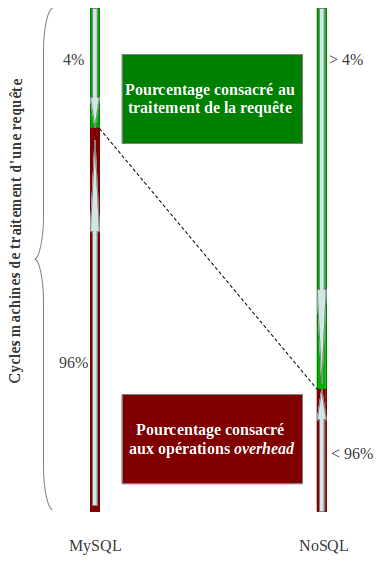
\includegraphics[scale=0.3]{\DIR/img/SQLvsNoSQL.png}	
        \caption{Répartitions des cycles machines \textsf{SQL} et \textsf{NoSQL}}
	\label{sqlvsnoql}
  \end {figure}    
\noindent
Toujours en quête de performance et comme mentionné à la section \ref{carac}, 
le \textsf{NoSQL} a renoncé à de la « \textsf{consistance forte} » pour de la « \textsf{consistance éventuelle} ». Il justifie ce choix par le théorème de \textsf{CAP} pendant que les \textsf{SGBDR} défendent systématiquement toutes les propriétés \textsf{ACID} dont la « \textsf{consistance forte} ». Ceci n'est pas sans compromis, notamment 
pour la reprise sur erreurs. 
\textsf{Michael Stonebraker} explique clairement sur 8 cas d'erreur,  
les enjeux du choix
des propriétés \textsf{CAP}\cite{MichaelStonebraker2}. Je me limiterai seulement à
3 cas d'erreur. Le but étant de mettre en relief les limites d'une « \textsf{consistance éventuelle} »
et d'exhiber deux situations qui rendent impossible la propriété \textsf{A} de \textsf{CAP} défendue par la mouvance \textsf{NoSQL}.
%===========================================================
%     Illustration enjeux du choix de AP dans CAP
%===========================================================
\def\exempleA{We assume a typical hardware model of a
collection of local processing and storage nodes assembled into a cluster using LAN networking.
The clusters, in turn, are wired together using WAN networking.
Let’s start with a discussion of what causes errors in databases:}

\def\exemple{Dans l'illustration qu'il a utilisé, \textsf{Michael Stonebraker} a considéré un ensemble de clusters interconnectés via un réseau \textsf{WAN}. 
Les nœuds à l'intérieur d'un cluster utilisent le \textsf{LAN} pour échanger. Ci-dessous trois cas d'erreur possibles:}

\def\casaA{Application errors. The application performed one or more incorrect updates. Generally, this is
not discovered for minutes to hours thereafter. The database must be
backed up to a point before the offending transaction(s), and
subsequent activity redone.}

\def\casa{Erreur au niveau de la couche application. Une application effectue une ou plusieurs mises à jour incorrectes. De telles erreurs ne sont généralement pas détectées dans les minutes qui suivent afin de revenir sur une version précédente de la base avant les mises à jour incorrectes.}

\def\casbA{Repeatable DBMS errors. The DBMS crashed at a processing node. Executing the same
transaction on a processing node with a replica will cause the backup
to crash. These errors have been termed Bohr bugs.}

\def\casb{Les erreurs reproductibles. Par exemple, une transaction fait planter le serveur principal. 
La même transaction fait tomber tous les autres serveurs copies qui vont servir de relais. 
Ces erreurs sont connues sous le nom de « \textsf{Bohr bugs} ».}

\def\cascA{\sf A disaster. The local cluster is wiped out by a flood, earthquake, etc. The cluster no longer exists.}

\def\casc{\sf Une catastrophe. Un cluster local est entièrement détruit.}

\def\commentA{First, note that errors 1 and 2 will cause problems with any high availability scheme. In these two
scenarios, there is no way to keep going; i.e., availability is
impossible to achieve. Also, replica consistency is meaningless; the
current DBMS state is simply wrong. Error 7 will only be recoverable
if a local transaction is only committed after the assurance that the
transaction has been received by another WAN-connected cluster. Few
application builders are willing to accept this kind of
latency. Hence, eventual consistency cannot be guaranteed, because a
transaction may be completely lost if a disaster occurs at a local
cluster before the transaction has been successfully forwarded
elsewhere. Put differently, the application designer chooses to suffer
data loss when a rare event (such as a disaster) occurs, because the
performance penalty for avoiding it is too high.}

\def\comment{Les deux premiers cas d'erreur conduisent la base dans un état incohérent. Ils affectent la disponibilité des données. Dans de telles situations, il est impossible de garantir la disponibilité des données même après avoir renoncé à de la consistance forte. Le troisième cas d'erreur montre les limites de
la consistance éventuelle. Les données ne pourront être récupérées que
si la transaction a été propagée sur un autre cluster avant la
catastrophe. Le temps de latence imposé par la consistance éventuelle
entre les mises à jour est donc problématique.}

\begin{center}
\begin{tabular}{p{1.7cm} p{12cm}}
\multicolumn{2}{p{14cm}}{\sf \exemple}\\&\\  
{\bf Cas 1} & \textsf{\casa}\\~&~\\ {\bf Cas 2}
& \textsf{\casb}\\~&~\\ {\bf Cas 3} & \textsf{\casc}\\
\end{tabular}
\end{center}
\noindent \comment
\\
\\
Pour finir, un paramètre à prendre en compte et pour ainsi reprendre la pensée de \textsf{Ted Dziuba},
est que contrairement aux solutions \textsf{NoSQL}, les \textsf{SGBDR} sont matures et ont par conséquent 
``une liste de limitations et de bugs connus''\cite{DieNosql}. L'utilisateur d'une \textsf{SGBDR} classique 
est plus ou moins rassuré parce qu'il sait à quoi s'en tenir. 


\section{Échange entre \textsf{SQL} et \textsf{NoSQL}}
Pour profiter des performances d'un \textsf{NoSQL}, il est essentiel
de définir à l'avance la nature et la représentation faite des données.
L'utilité et le choix du \textsf{NoSQL} doit principalement
réposer de la représentation des données. Adopter le \textsf{NoSQL} à
cause de la volumétrie ne garantit pas la performance et surtout la 
base perd l'intégrité qu'offre le modèle rélationnel.  
\\ 
\\ 
Les « \textsf{NoSQL} » offrent une autre façon
de représenter les données pour faciliter les accès et mises à jour des
données afin de gagner en performance. Le \textsf{NoSQL} n'est pas 
là pour remplacer systématiquement le  \textsf{SQL}. Pour la gestion des données 
organisée en tables, la structure des \textsf{SGBDR} y est exclusivement
dédiée. Cependant certaines solutions \textsf{NoSQL}, à l'image de \textsf{MongoDB}, ont
exhibé une charte de correspondance entre leurs composants et les composants \textsf{BDDR} 
\footnote{Database, Table, Index, colonne, clé
  primaire ...}. \textsf{MongoDB} a également mis
en place une charte de traduction requête \textsf{SQL} / requête
\textsf{MongoDB}.
\\
\\
\textsf{SQL} d'une part, \textsf{NoSQL} d'autre part, l'un n'exclut pas l'autre.
Tout dépend de l'usage qu'on compte en faire ou du profit qu'on
souhaite en tirer. Pour profiter à la fois du \textsf{NoSQL} et du \textsf{SQL}, il est très commun
de les faire cohabiter et de stocker
les données dans l'un ou dans l'autre en fonction des caractéristiques de 
celles-ci. C'est ce que fait d'ailleurs \textsf{Google} qui
même après avoir mis en place sa solution
propriétaire \textsf{BigTable} utilise \textsf{MySQL}
notamment pour son programme publicitaire \textsf{AdWords}, sa
principale source de revenue, et qui utilise d'énormes quantités de
données. Cependant imaginer un protocole d'échange entre \textsf{SQL}
et \textsf{NoSQL} peut s'avérer très fastidieux dans la mesure où les
deux conçoivent les données très différemment.
\\
\\
Il existe une solution \textsf{Open Source} permettant des échanges
\textsf{SQL}/\textsf{NoSqL}: \textsf{Sqoop} ou « SQL To Hadoop
». \textsf{Hadoop}\index{Sqoop} est un assemblage de plusieurs
sous-projet avec à la base un système de
fichier \textsf{HDFS}\footnote{Hadoop Distributed File System}
et \textsf{HBASE} pour le stockage. Développé en \textsf{java}, sous
la direction de la fondation \textsf{Apache} et destiné aux
applications distribuées, sa structure de stockage \textsf{HBASE} est
un x\textsf{NoSQL} orienté colonnes. \textsf{Sqoop} charge
une table ou toute la base en système de fichiers \textsf{HDFS} en
fonction des options d'importation spécifiées et génère aussi des
classes \textsf{java} correspondantes aux tables de la bases, ainsi
que des objets correspondants aux lignes pour permettre d'interagir
avec les données importées.
\begin {figure}[H]
       \centering
        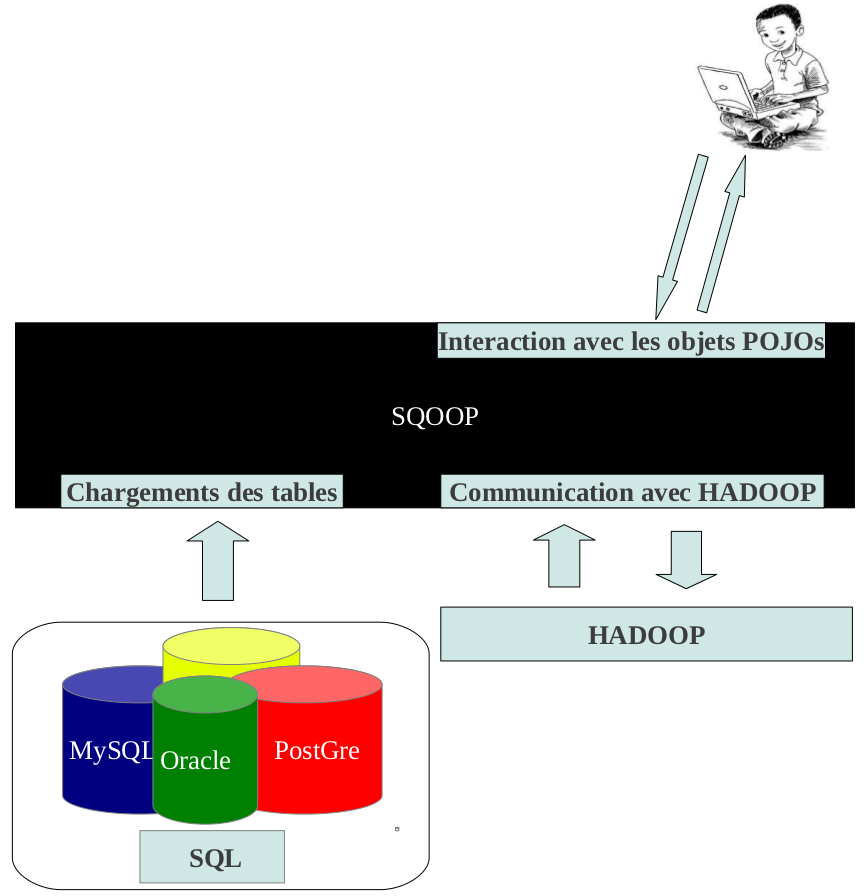
\includegraphics[scale=0.2]{\DIR/img/sqoop.png}	
        \caption{Fonctionnement de \textsf{SQOOP}}
	\label{sqoop}
  \end {figure}    
\noindent
Mise à part \textsf{Sqoop} qui est une solution pour \textsf{Hadoop}
d'échange avec le \textsf{SQL}, le framework
\textsf{spring} intègre des modules \textsf{Data access}\cite{springsource} permettant 
de faire persister des objets \textsf{POJO}\footnote{Acronyme de \textsf{P}lain \textsf{O}ld \textsf{J}ava \textsf{O}bject désignant les objets java simples n'héritant d'aucune classe et n'implémentant aucune interface } dans des \textsf{BDD NoSQL}. 
En exemple, le module \textsf{Spring Data MongoDB} permet de faire persister
les données dans \textsf{MongoDB}. Avec \textsf{spring} il est alors possible
d'effectuer une échange en deux temps:
\begin{enumerate}
\item D'abord transformer les données dans la \textsf{BDDR} en des objets 
      \textsf{POJO} par le biais de module déjà existant
      comme \textsf{hibernate, toplink, iBatis}...
\item Puis faire persister les objets \textsf{POJO} dans la base \textsf{NoSQL} par le biais du module 
      \textsf{Data access} dédié.    
\end{enumerate} 
Cependant il faut changer de module \textsf{Data access} à chaque fois
qu'il faut changer de \textsf{BDD NoSQL}. Il est difficile de mettre
en place une standardisation des interfaces dans la mesure où
chaque \textsf{BDD NoSQL} vient avec son propre langage de requête.
\begin {figure}[H]
       \centering
        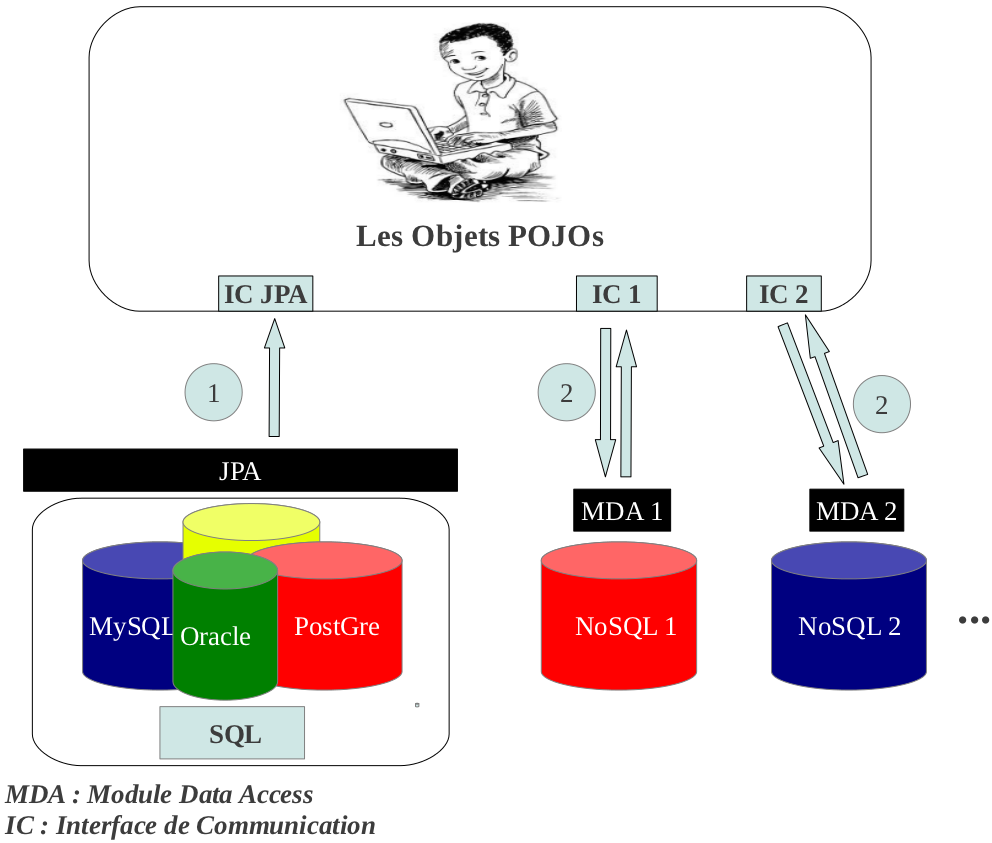
\includegraphics[scale=0.2]{\DIR/img/spring.png}	
        \caption{Possibilité d'échange \textsf{SQL/NoSQL} avec \textsf{spring}}
	\label{spring}
\end {figure}


\section{Système de Rootage intelligent entre \textsf{SQL} et \textsf{NoSQL}}
Il n'y vraiment pas grand chose à ce sujet. Ce qui ressort à chaque fois ce sont les motivations pour adopter le \textsf{NoSQL} qui sont: quantités de données et environnement distribué à fort trafic.



\chapter{Choix des \textsf{NoSQL mongoDB} et \textsf{cubeLaBRI}}
\section{Le \textsf{NoSQL mongoDB}}
\noindent \textbf{Norme de stockage}: Le \textsf{BSON} un dérivé binaire du \textsf{JSON} qui offre un bon rapport entre la place occupée et la rapidité de parsing notamment en intégrant la taille de chaque entrée pour pouvoir passer à la suivante si la clé ne correspond pas.
\\
\\
\textsf{replicaset et shards} sont deux notions fondamentales dans la distribution des données de MongoDB.

\section{Le \textsf{NoSQL} \textsf{cubeLaBRI}}
\input{src/cube}

\chapter{Les tests de charge}
\section{Tests de charge sur \textsf{mongoDB}}
\section{Tests de charge sur \textsf{cubeLaBRI}}
\section{Le choix definitif d'\textsf{EVOLLIS} de la solution \textsf{NoSQL}}

\chapter{Pilote du \textsf{NoSQL} xxxx pour \sf  EVOLLIS}

\addcontentsline{toc}{chapter}{Conclusion}
% 


\nocite{wikiNoSQL}

%\bibliographystyle{unsrt}
\bibliography{bibliographie}

%%%%%% Liste des annexes %%%%%%%%%%
\part{Annexes}
\appendix
\chapter{Les propriétés \textsf{ACID}}\label{acid}
Les propriétés \textsf{ACID} permettent à un \textsf{SGBD} d'effectuer
des transactions. Par transaction, il faut comprendre une suite
d'opérations qui font passer la \textsf{BDD} d'un état antérieur à un
état postérieur. Les états intermédiaires entre les états avant la
transaction et après la transaction ne sont pas visibles. Ses
propriétés sont les suivantes:

\paragraph{Atomicité:} la suite d'opérations constituant une transaction 
est indivisible. La transaction est entièrement effectuée ou pas du tout. 
Il y a annulation de toute la transaction lorsqu'une des opérations échoue.
S'il est question de modifier une série de valeurs et qu'une modification
échoue alors toutes les valeurs déjà modifiées reprennent leurs anciennes
valeurs. 

\paragraph{Cohérence:} quelque soit l'opération effectuée, la base doit garder
un état cohérent. Toute transaction qui viole par exemple une règle d'intégrité 
échoue. Après la fusion de deux tables, les entrées doivent toutes 
avoir des identités différentes. Si ce n'est pas le cas alors la fusion n'est 
pas effectuée.

\paragraph{Isolation:} chaque transaction est isolée de sorte à ce qu'elle est 
seule peut voir les modifications pendant son exécution. Toute
transaction enclenchée en parallèle d'une autre voit la version des
données antérieure à celle-ci.  Il existe 4 niveaux d'isolation
définis dans le standard \textsf{ANSI/ISO SQL}:
\begin{enumerate}
\item \textsf{Uncommited read ou lectures des données non validées}.
  Ce niveau est le niveau d'isolation le plus léger. Avec un tel
  niveau d'isolation le système se comporte comme s'il n'y en avait
  pas. Les modifications apportées par une transaction non validée
  sont visibles.

\item \textsf{Commited read ou lecture des seules données
  validées}. Les modifications lors d'une transaction ne sont visibles
  que lorsqu'elle termine.  Cependant lors d'une transaction une
  donnée peut changer sans que la transaction en cours en soit
  responsable. Ceci peut arriver, par exemple, lorsqu'une transaction
  en parallèle termine et que ses modifications sont validées.

\item \textsf{Repeatable read ou lecture répétée}. Ce niveau
  fonctionne comme le niveau précédent à la seule différence que
  durant son exécution, une transaction ne voit pas les mises à jour
  effectuées par d'éventuelles transactions qui se sont exécutées en
  parallèle. D'où « \textsf{repeatable read} » pour souligner que pendant une
  transaction, une donnée aura toujours la même valeur en
  lecture si elle n'est pas modifiée par la transaction elle-même.
  Cependant tout nouveau rajout validé de données au système par une
  transaction qui a terminé est visible par toute autre transaction en
  cours.

\item \textsf{Serializable ou sérialisable}. Ce niveau est le niveau
  d'isolation le plus poussé. Le système se comporte comme s'il n'y
  avait qu'une transaction à la fois. Pendant son exécution une
  transaction ne voit ni les mises à jour, ni les rajouts de données
  au système des autres transactions. D'où « \textsf{serializable} » pour
  mettre en relief le caractère d'exécution en série des transactions
  plutôt qu'en parallèle.
\end{enumerate}

\paragraph{Durabilité:} dès lors qu'une transaction est validée, aucune défaillance
du système ne pourra conduire à l'annulation de celle-ci. Les modifications liées à
une transaction validée perdurent et ne sont jamais remises en cause.

\end{document}
